%-------------------------------------------------------------------------------
\subsection{Calcul différentiel}
%-------------------------------------------------------------------------------

\todo{Voir L3 Bio SU : TD1, exercice 2}

%-------------------------------------------------------------------------------
\subsection{Systèmes dynamiques en dimension 1}
%-------------------------------------------------------------------------------

\todo{Voir L3 Bio SU : TD2, exercice 1}

\exemple{[Exercice 2, TD2, L2 Bio SU]
  On considère le système
  $$
  \dot y = - y^3 + 7 y^2 - 14 y + 8.
  $$
  Ses points stationnaires sont les racines du polynôme $P(y) = - y^3 + 7 y^2 - 14 y + 8$, donc $y_1 = 1$ fait partie, donc
  $$
  P(y) = (y-1) (-y^2 + 6y + 8),
  $$
  et les deux racines de $-y^2 + 6y + 8$ sont $2$ et $4$. Les points stationnaires du système sont donc 
  $$
  y_1 = 1, \qquad y_2 = 2, \qquad y_3 = 4.
  $$
  Leur stabilité est donné par la dérivée de $P$:
  $$
  P'(y) = -3y^2 + 14 y - 14,
  $$
  soit
  $$
  P'(y_1) = -3, \qquad P'(y_2) = 2, \qquad P'(y_3) = -6.
  $$
  $y_1$ et $y_3$ sont donc des équilibres stables, et $y_2$ un équilibre instable.
  $$
  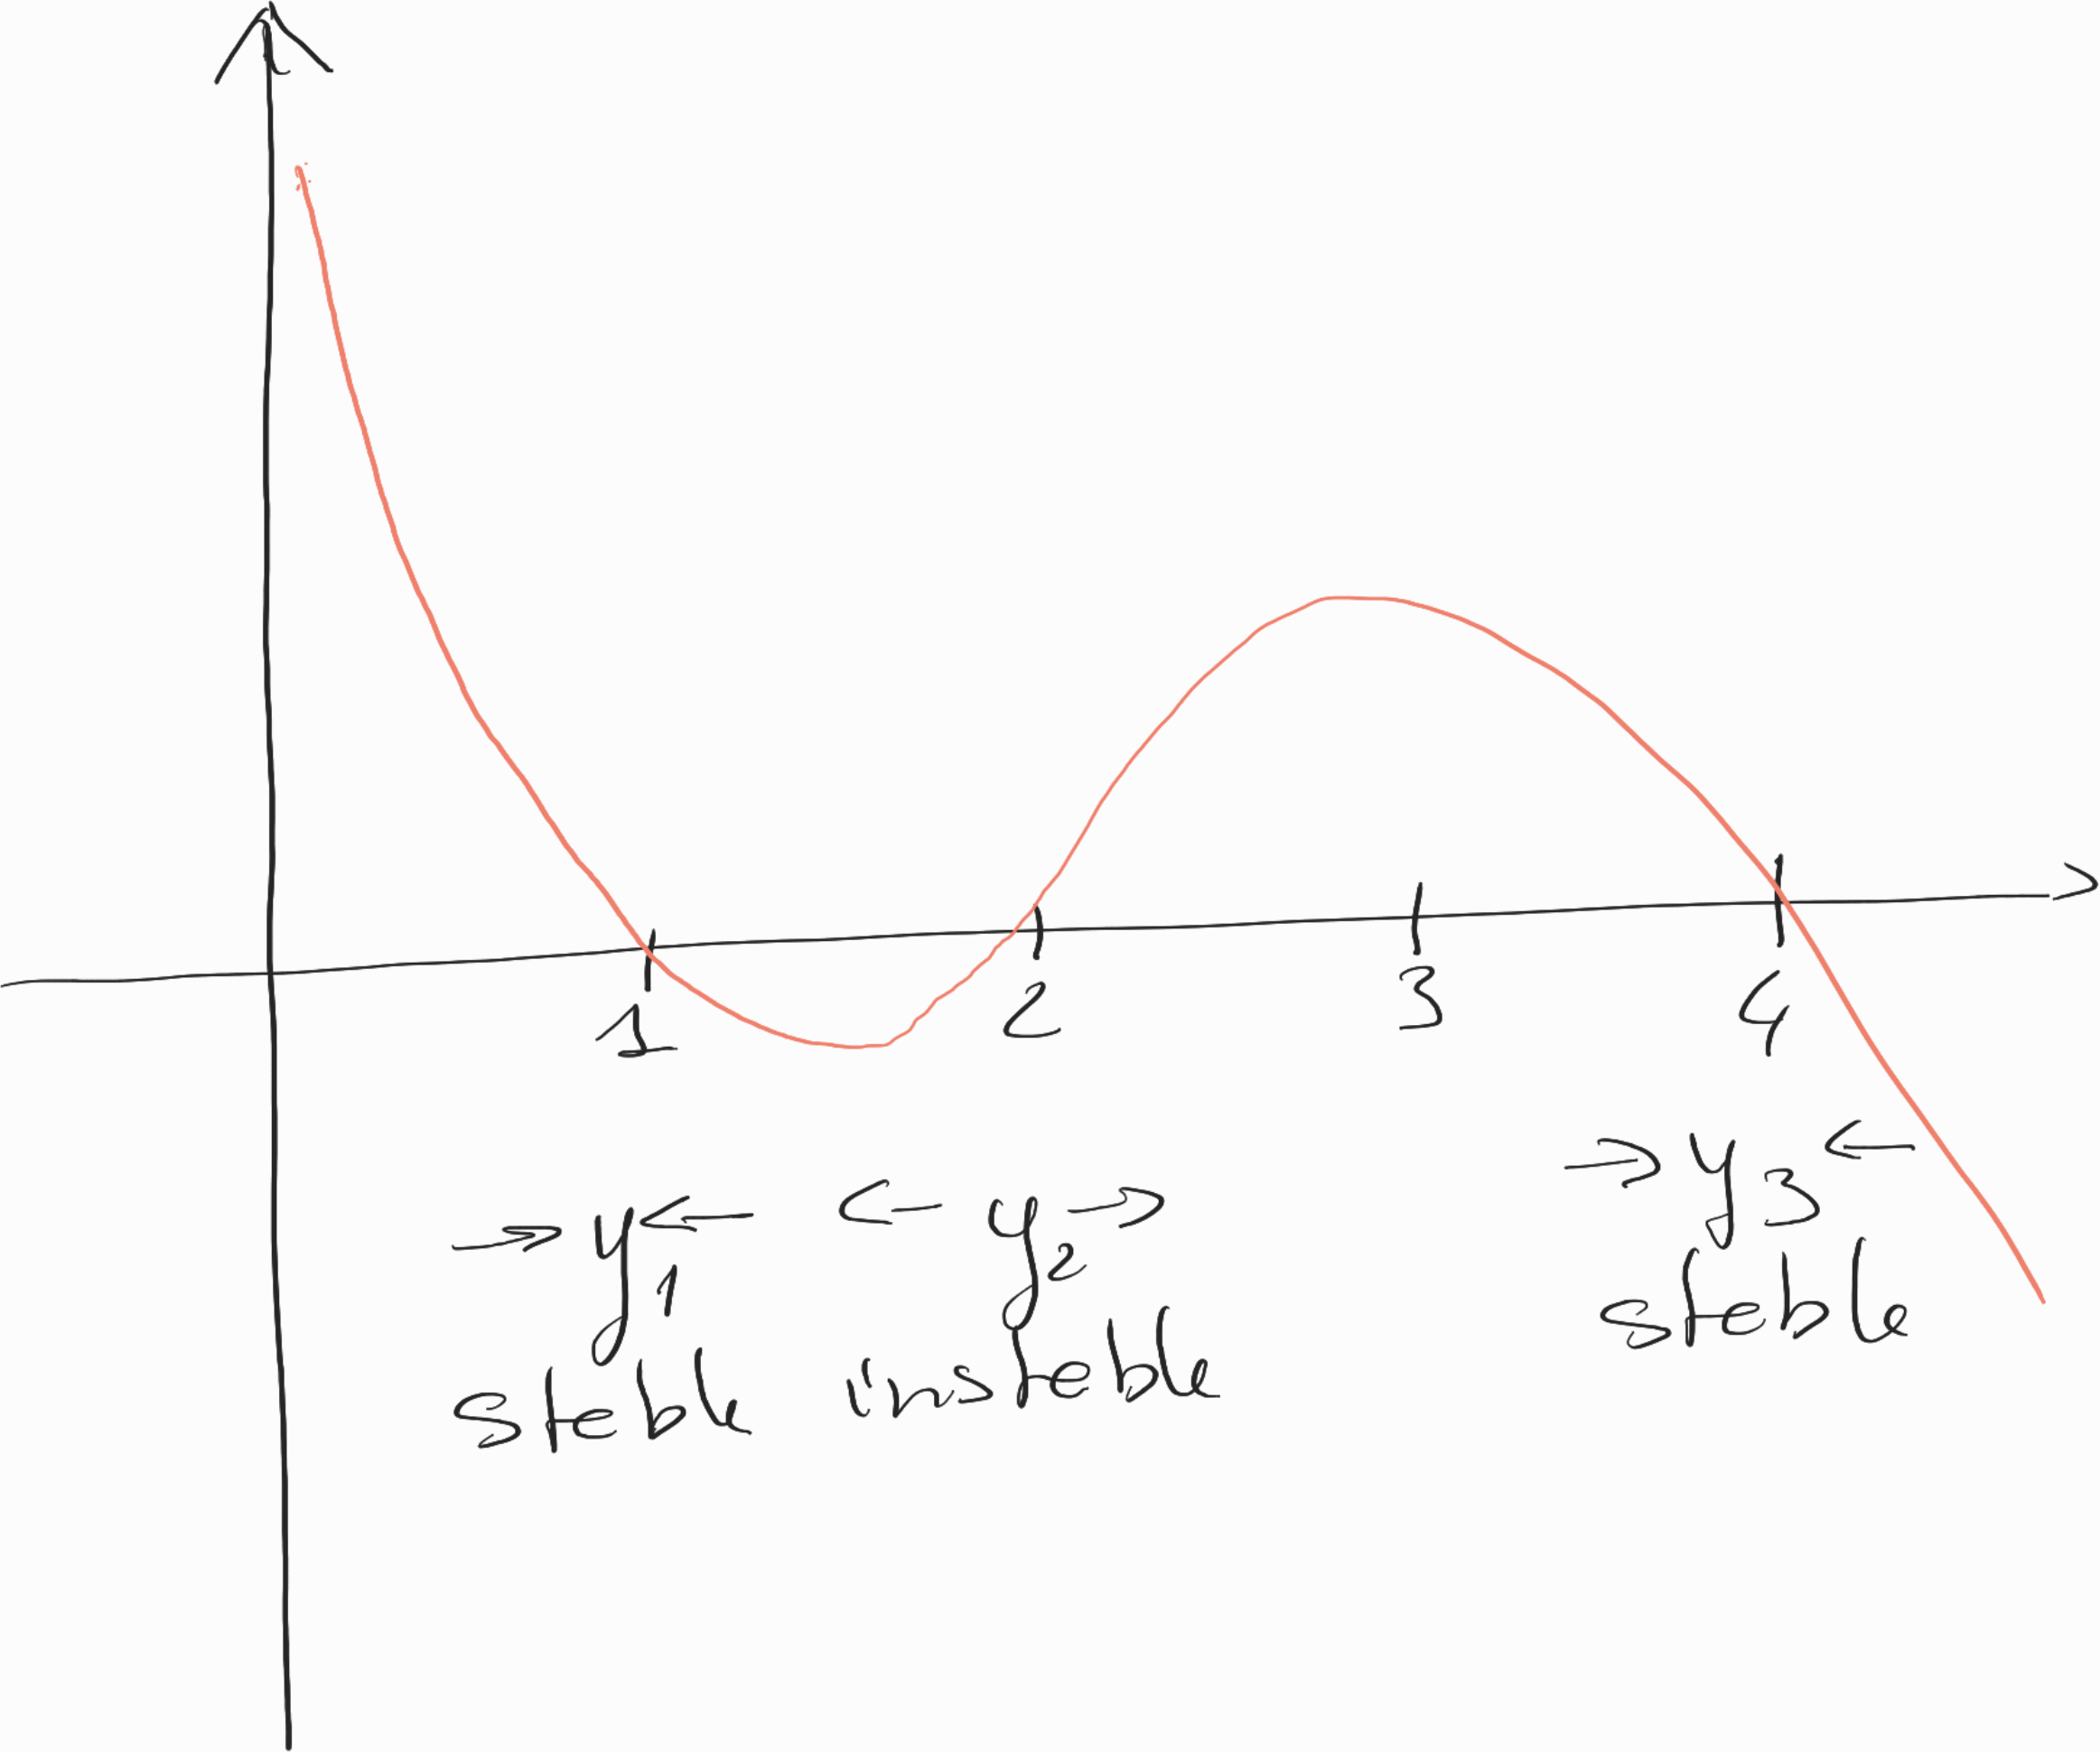
\includegraphics[width=.5\textwidth]{TD-SUbioL3-TD2Exo2}
  $$
}

%-------------------------------------------------------------------------------
\subsection{Systèmes dynamiques en dimension 2}
%-------------------------------------------------------------------------------

%-------------------------------------------------------------------------------
\begin{exercise}[Système dynamique] \label{SystDyn-Lineaire}
  On considère le système dynamique suivant
  $$
  \left\{\begin{array}{rcl}
         \dot x & = & -a_1 x + b_1 y + c_1 \\ 
         \dot y & = & -a_2 x + b_2 y + c_2
         \end{array}\right.
  $$
  où tous les coefficients constants sont strictement positifs.
  \begin{enumerate}
   \item À quelle condition y a-t-il un unique équilibre ? Lorsque c’est le cas, à quelle condition est-il stable ?
   \item Lorsqu’il n’existe pas d’équilibre unique, représenter les deux isoclines (c'est à dire les ensemble de points ou s'annule $\dot x$ d'une part et $\dot y$ d'autre part). Y a-t-il une infinité d’équilibres ou aucun équilibre ?
   \item Représenter les orbites dans le plan de phase.
  \end{enumerate}
\end{exercise}

\solution{\todo{}}

%-------------------------------------------------------------------------------
\begin{exercise}[Système dynamique] \label{SystDyn-Quadratique}
  On considère le système dynamique d’activation réciproque suivant avec compétition intraspécifique
  $$
  \SR{
  \left\{\begin{array}{rcl}
         \dot x & = & r y - cx^2 \\ 
         \dot y & = & r x - cy^2 
         \end{array}\right.
  }{
  \left\{\begin{array}{rcl}
         \dot x & = & a y - x^2 \\ 
         \dot y & = & a x - y^2 
         \end{array}\right.
  }
  $$
  où $r$ et $c$ sont deux constantes strictement positives.
  \begin{enumerate}
   \item Donner la valeur $(x^*, y^*)$ de l’unique équilibre non trivial\footnote{'Trivial' signifie à la fois évident et sans intérêt. En l'occurrence, le point d'équilibre trivial est le point $(0, 0)$.} de ce système dans le quadrant positif. Quel est l’autre équilibre ?
   \solution{\todo{} $x^* = y^* = a$}
   \item Donner la nature de chacun de ces deux équilibres.
   \solution{\todo{} $(0, 0) =$ point selle, $(a, a) =$ instable.}
   \item Que se passe-t-il si $x(0) = y(0) > 0$ ? Représenter l’allure des trajectoires dans le plan de phase. 
  \solution{\todo{}}
  \end{enumerate}
\end{exercise}

